\documentclass[UTF8]{ctexart}
\usepackage{../Zhihu}
\title{数字电路学习笔记(一):前言}
\begin{document}
\maketitle
决定写一系列关于数字电路的文章,整理一下过去几个月内本人自学的相关知识,从一个高中生的角度讲讲我对知识点的理解,算是一种巩固练习。限于知识水平,许多内容可能没有真正理解,如果有大佬路过,也欢迎提出改进意见,谢谢!

\divider

\section*{一、什么是数字电路?}
我们从一道经典的初中物理题开始:

\begin{quote}
某档案室有三把钥匙,分别由主任与两个保管员保管。主任的钥匙可以直接开门,而两个保管员的钥匙则只有同时插入才能开门。档案室大门还有一个防盗装置,激活时无论什么钥匙都无法开门。试画出电路图,用电键表示钥匙孔与防盗装置,马达表示门锁。
\end{quote}

当然,题目本身并没什么难度,任何一个受过良好的九年义务教育的同学都应该能完成:

\begin{figure}
    \begin{circuitikz}
        \draw (2,0) 
            to[battery,*-] (0,0);
        \draw (2,0)
            to[short] (2,0.5)
            to[normal open switch={保管员A}] (4,0.5)
            to[normal open switch={保管员B}] (6,0.5)
            to[short,-*] (6,0);
        \draw (2,0)
            to[short] (2,-0.5)
            to[normal open switch={主任}] (6,-0.5)
            to[short] (6,0)
            to[short] (7,0)
            to[short] (7,3)
            to[Telmech] (0,3)
            to[R] (0,0);
        \draw (2,3)
            to[short,*-] (2,4)
            to[normal open switch={防盗系统}] (5,4)
            to[short,-*] (5,3);
    \end{circuitikz}
\end{figure}

但是,这道题目看似沙雕,实则暗含了数字电路的思想!我们重新审视一下这道题:

\begin{quote}
当“主任的钥匙插入”\textbf{\textit{或者}}“‘档案保管员A的钥匙插入’\textbf{\textit{而且}}‘档案保管员B的钥匙插入’”\textbf{\textit{而且}}“防盗装置\textbf{\textit{未}}开启时,门锁打开
\end{quote}

我们把所有可能的情况列出来看看:

\begin{figure}
    \begin{tabular}{|c|c|c|c|c|}\hline\rowcolor{lightgray}
        主任   &保管员A&保管员B & 防盗装置&门锁\\\hline
        未就位 &未就位 & 未就位 & 关闭   &关闭\\\hline
        未就位 &未就位 & 未就位 & 开启   &关闭\\\hline
        未就位 &未就位 &   就位 & 关闭   &关闭\\\hline
        未就位 &未就位 &   就位 & 开启   &关闭\\\hline
        未就位 &  就位 & 未就位 & 关闭   &关闭\\\hline
        未就位 &  就位 & 未就位 & 开启   &关闭\\\hline
        未就位 &  就位 &   就位 & 关闭   &开启\\\hline
        未就位 &  就位 &   就位 & 开启   &关闭\\\hline
        就位   &未就位 & 未就位 & 关闭   &开启\\\hline
        就位   &未就位 & 未就位 & 开启   &关闭\\\hline
        就位   &未就位 &   就位 & 关闭   &开启\\\hline
        就位   &未就位 &   就位 & 开启   &关闭\\\hline
        就位   &  就位 & 未就位 & 关闭   &开启\\\hline
        就位   &  就位 & 未就位 & 开启   &关闭\\\hline
        就位   &  就位 &   就位 & 关闭   &开启\\\hline
        就位   &  就位 &   就位 & 开启   &关闭\\\hline
    \end{tabular}
\end{figure}

进一步抽象化,注意到这个逻辑中包含了四个“自变量”事件,可以分别用$A$、$B$、$C$、$D$表示;而它们则操纵着一个“因变量”事件,用$X$表示;再定义“1”为开关闭合或马达运转,“0”则相反:

\begin{figure}
    \begin{tabular}{|c|c|c|c|c|}\hline\rowcolor{lightgray}
        $A$   &$B$&$C$ & $D$&$X$\\\hline
        0 &0 & 0 & 0   &0\\\hline
        0 &0 & 0 & 1   &0\\\hline
        0 &0 & 1 & 0   &0\\\hline
        0 &0 & 1 & 1   &0\\\hline
        0 &1 & 0 & 0   &0\\\hline
        0 &1 & 0 & 1   &0\\\hline
        0 &1 & 1 & 0   &1\\\hline
        0 &1 & 1 & 1   &0\\\hline
        1 &0 & 0 & 0   &1\\\hline
        1 &0 & 0 & 1   &0\\\hline
        1 &0 & 1 & 0   &1\\\hline
        1 &0 & 1 & 1   &0\\\hline
        1 &1 & 0 & 0   &1\\\hline
        1 &1 & 0 & 1   &0\\\hline
        1 &1 & 1 & 0   &1\\\hline
        1 &1 & 1 & 1   &0\\\hline
    \end{tabular}
\end{figure}

到这里,我们已经列出了一个叫“真值表”的东西。其实,它还可以被化为更加抽象的函数形式——类似$(A+BC)\cdot D'$这样——在以后,会看到它是如何在电路设计中起到关键作用的。

总结一下,首先有四个数字输入信号(它们的幅值和时间都是离散的),通过一系列“黑箱操作”逻辑或运算规则,把四个自变量进行运算,得出了一个因变量——事实上,这就是数字电路。

\section*{二、为什么要有数字电路?}
数字电路,实际上就是计算机的基础——计算机本质上,就是通过对一系列由0和1组合的量进行运算,得出结果的。而再弱化一点,哪怕是对几个指示灯的控制,或者简单的饮料机,也会用到逻辑电路。

从古至今,人类都面临着一个相同的问题:懒惰。人类几乎是天生地不想去做重复的工作,因而发明了各种各样的工具替代我们完成这些任务——比如印刷术,比如交通工具,比如水轮磨坊。这些不仅将人们从低价值的劳动中解放出来,还极大提高了社会生产效率。可以说,是懒惰促进了社会的进步。(误)

而数字电路,则就是人类大脑的扩展。在刚才的例子中,我们完全可以派一个尽心尽责的保安大叔在门口负责大门开闭——但谁能保证,他就不会出错呢?或者退一步讲,任何一个人日复一日地干这样无聊的工作,效率肯定不会高吧?因此,数字电路就代替了这些人脑的机械的逻辑运算。无论是几百根管的真空管电路,还是上千万门级别的集成电路,归根结底都是起着类似的作用。而数字电路做成的小元件以一定的方式组合,就成了计算机的雏形。

但是,由于本人并不精于微电子,许多关于电路设计的理论都仅限于纸上谈兵,对于硬件的了解非常有限,因此也无法对电路本身的性能作出负责的评价。对于数字信号与模拟信号也未做太多说明,留至A-D转换部分(如果我坚持的到的话)再写。

\section*{三、为什么我要自学数电?}
惭愧的是,我一开始学习数电的目的,竟然是为了打游戏...

\begin{figure}
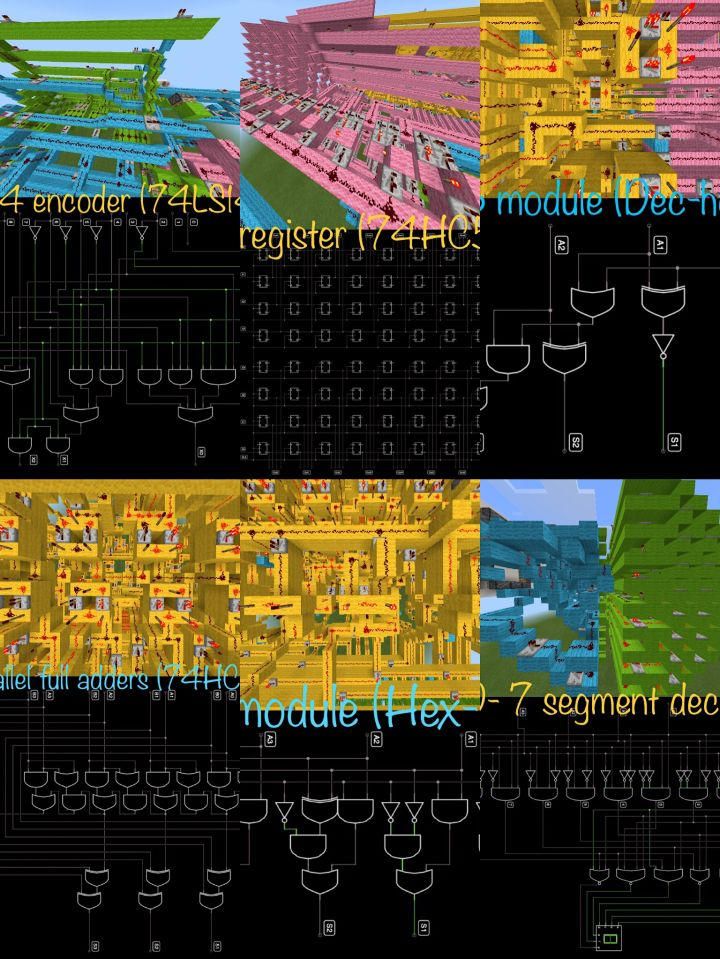
\includegraphics[width=10cm]{Fig1.jpg}
\caption*{奋战两个月的成果}
\end{figure}
Minecraft中提供了红石线与红石火把两种最基础的元件,分别可以作为或门和非门使用;而这两个门就可以组合出所有逻辑门,进而搭建出计算器、控制器之类的大型电路。因此,如果要在Minecraft中完全掌握红石技术,数字电路知识是必不可少的。

当然,随着我接触编程,渐渐意识到了计算机方面的基础知识(数电模电、组成原理、编译原理)对语言理解的必要性,因此更加需要学习。

那么,前言部分就这么结束了,让我们赶快进入正文。

\textit{最后的最后,既然来都来了,就捧个场呗?}
\end{document}